\section{Diskussion} 
\begin{frame}{Emner til diskussion}
    To overordnede emner:
    \begin{itemize}
        \item Hvorfor lave GT?
        \item Hvordan testes GT?
    \end{itemize}
\end{frame}

\begin{frame}{Ændringer i billedet}

    \begin{itemize}
        \setlength\itemsep{1em}
        \item Minimere antal ændringer i pixels
        \item For let at se i histogram
        \begin{itemize}
            \vspace*{1em}
            \setlength\itemsep{1em}
            \item<con@1->[$\times$] Ændring i pixelfarve
            \item<pro@1->[\checkmark] Ombytte AC-koefficienter
        \end{itemize}
    \end{itemize}
\end{frame}

% Grunden til cover og GT er lidt forskellige
% er pga. de få forces, der er.
% Hvis GT udelukkende havde brugt switches,
% havde histogrammerne været ens.
\begin{frame}{Ændringer i billedet}
    \begin{figure}
        \centering
        \begin{center}
        \subfigure[JPEG u. besked]{\label{fig:a}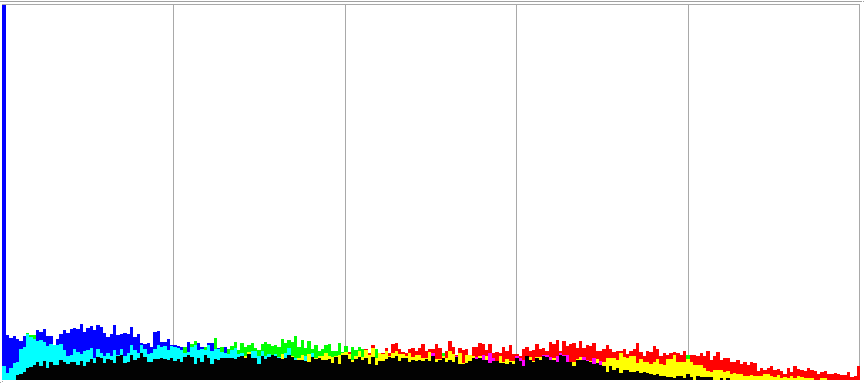
\includegraphics[width=.4\textwidth]{figures/gtOut2Histo.png}}
        \end{center}
        ~
        \subfigure[LSB m. besked]{\label{fig:b}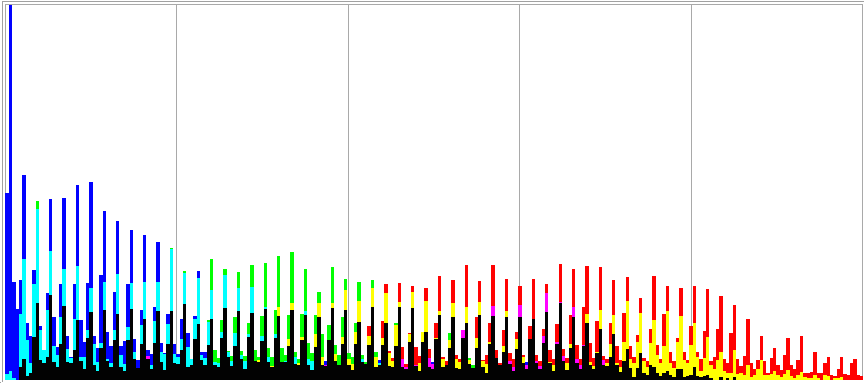
\includegraphics[width=.4\textwidth]{figures/lsbOutHisto.png}}
        ~
        \subfigure[GT m. besked]{\label{fig:c}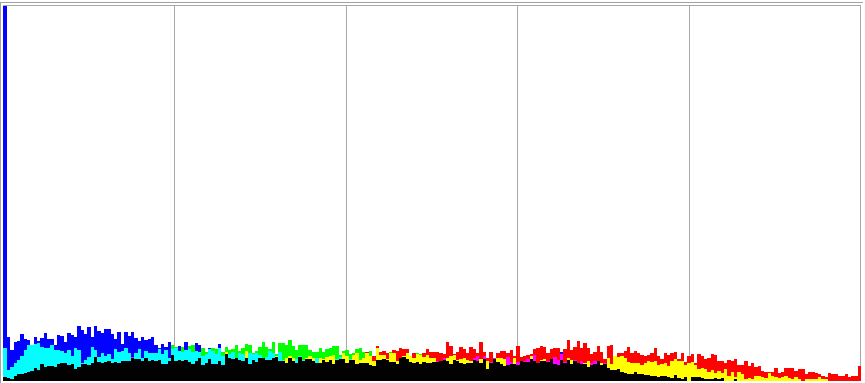
\includegraphics[width=.4\textwidth]{figures/gtOutHisto.png}}
        \caption{Samme besked, forskellige metoder}
    \end{figure}
\end{frame}

\begin{frame}{Testabilitet}
    \begin{itemize}
        \item Test-driven development ift. testing bagefter
        \item Usability testing
    \end{itemize}
\end{frame}
\begin{frame}[fragile]{Testabilitet}
    Mange private metoder
    \begin{itemize}
        \item Fleksibilitet %mht. implementering
        \item Lav testabilitet
    \end{itemize}
    \begin{itemize}
        \item<1-> \lstinline|PrivateObject| \& \lstinline|PrivateType|
        \item<2-> \ldots Eller udelukkende public?
    \end{itemize}
\end{frame}

\section{Konklusion}
\begin{frame}{Konklusion}
    Fokus på
    \begin{itemize}
        \item{\sout{Sociale medier} $\rightarrow$ Diskrethed}
        \item {Timeglasmodel}
        \item JPEG encoder
        \item Studieordning:
        \begin{itemize}
            \item\textcolor{green}{\checkmark} Problemafgrænsning
            \item\textcolor{green}{\checkmark} Model
            \item\textcolor{green}{\checkmark} Større program
            \item\textcolor{green}{\checkmark} Tests
            \item\textcolor{green}{\checkmark} Analysere problemorienteret projektarbejde
            \end{itemize}
    \end{itemize}
\end{frame}
